\documentclass{subfiles}

\begin{document}
    Zuerst kann man das verlauf des Potentials $V(x,y)$ zeichnen. Hier ist $m_{E}$ = 10 \cdot $m_{M}$.
    \begin{figure}[H]
        \centering
        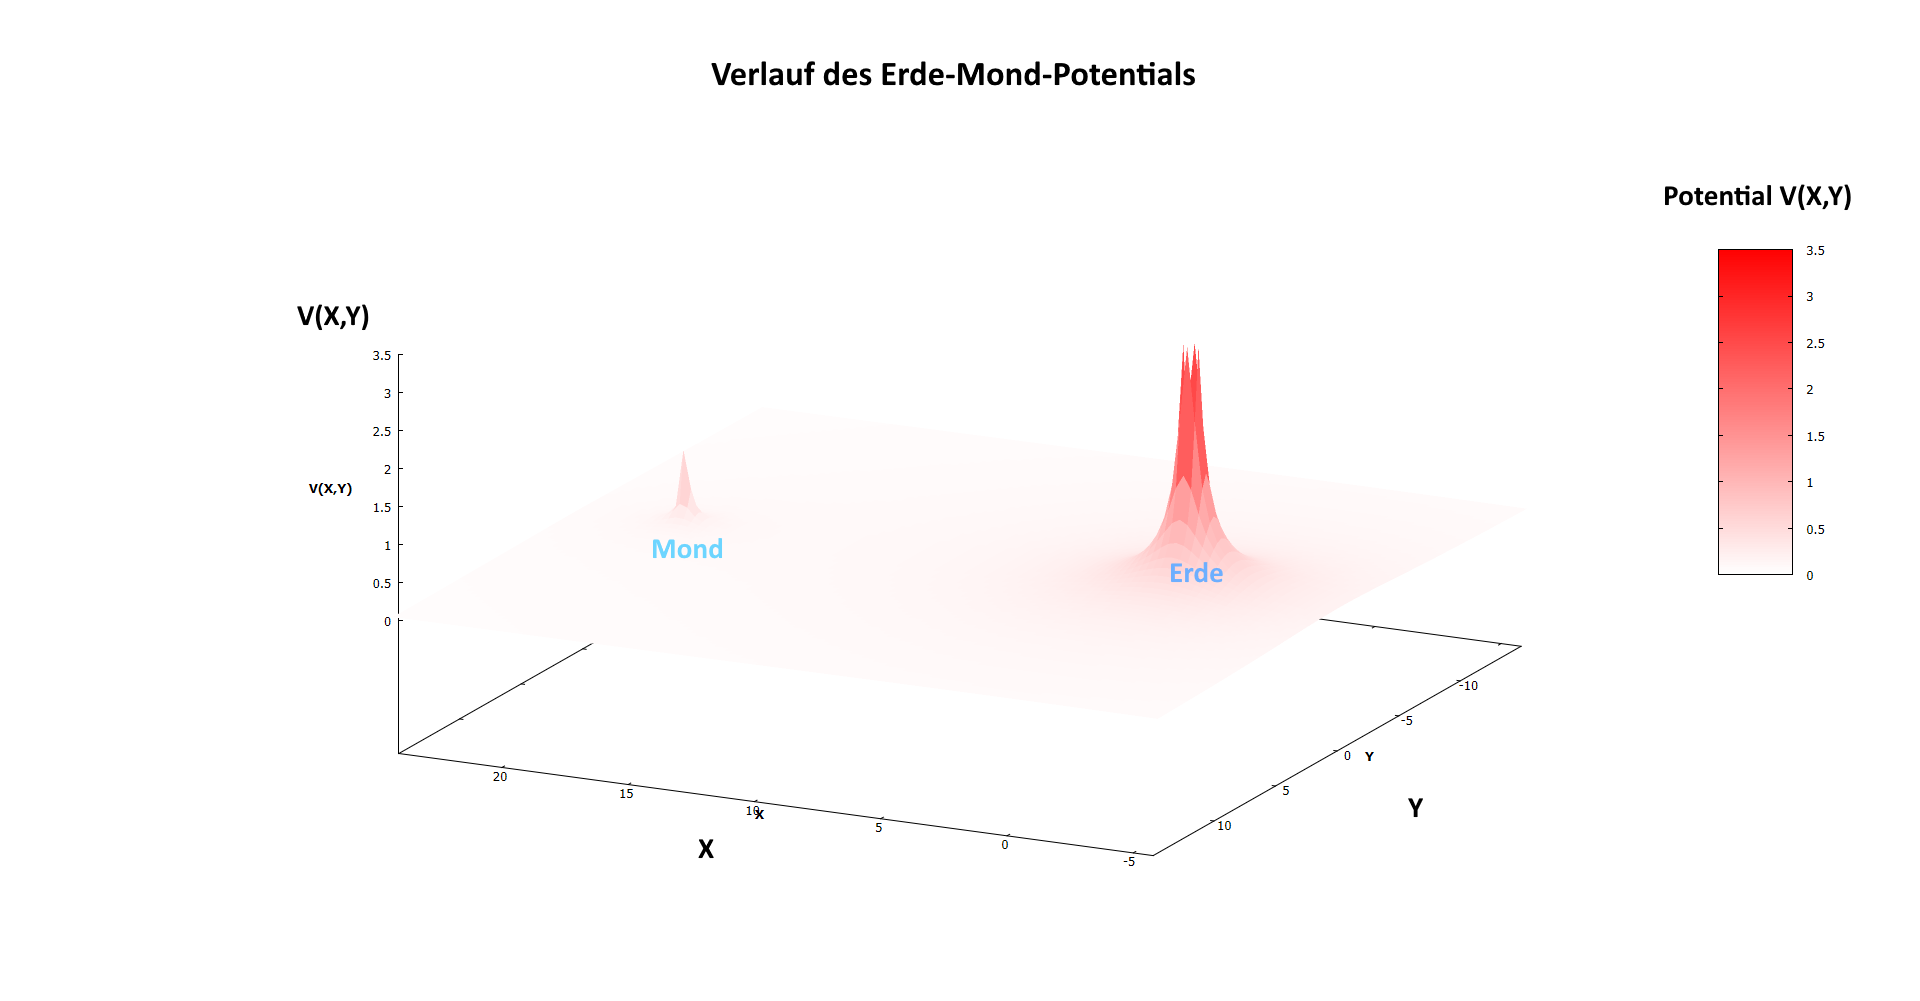
\includegraphics[width=0.8\textwidth]{../Ressource/PotentialVerlauf.png}
        \caption{Potentialverlauf}
        \label{fig:Potential}
    \end{figure}
    Für praktische Gründen sind die Abstände zwischen die Planetten viel kleiner. Hier sollte die Größenordnung $\num{e9}$m sein.\newline

    Wir haben uns aber während die Grundlagen Anteil für die kugelkoordinate Darstellung entschieden. Wir wählen eine Phase des Mondes
    $\Phi_M(t) = 0$ und ein Ellipsenparameter $a = 1$Abstand Mond-Erde. Weiter ist der Azimutal-Winkel gleich 0 gestellt, sodass wir eine Projektions
    des Potentialverlaufes auf die $x$-$y$-Ebene erhalten.
    \begin{figure}[H]
        \centering
        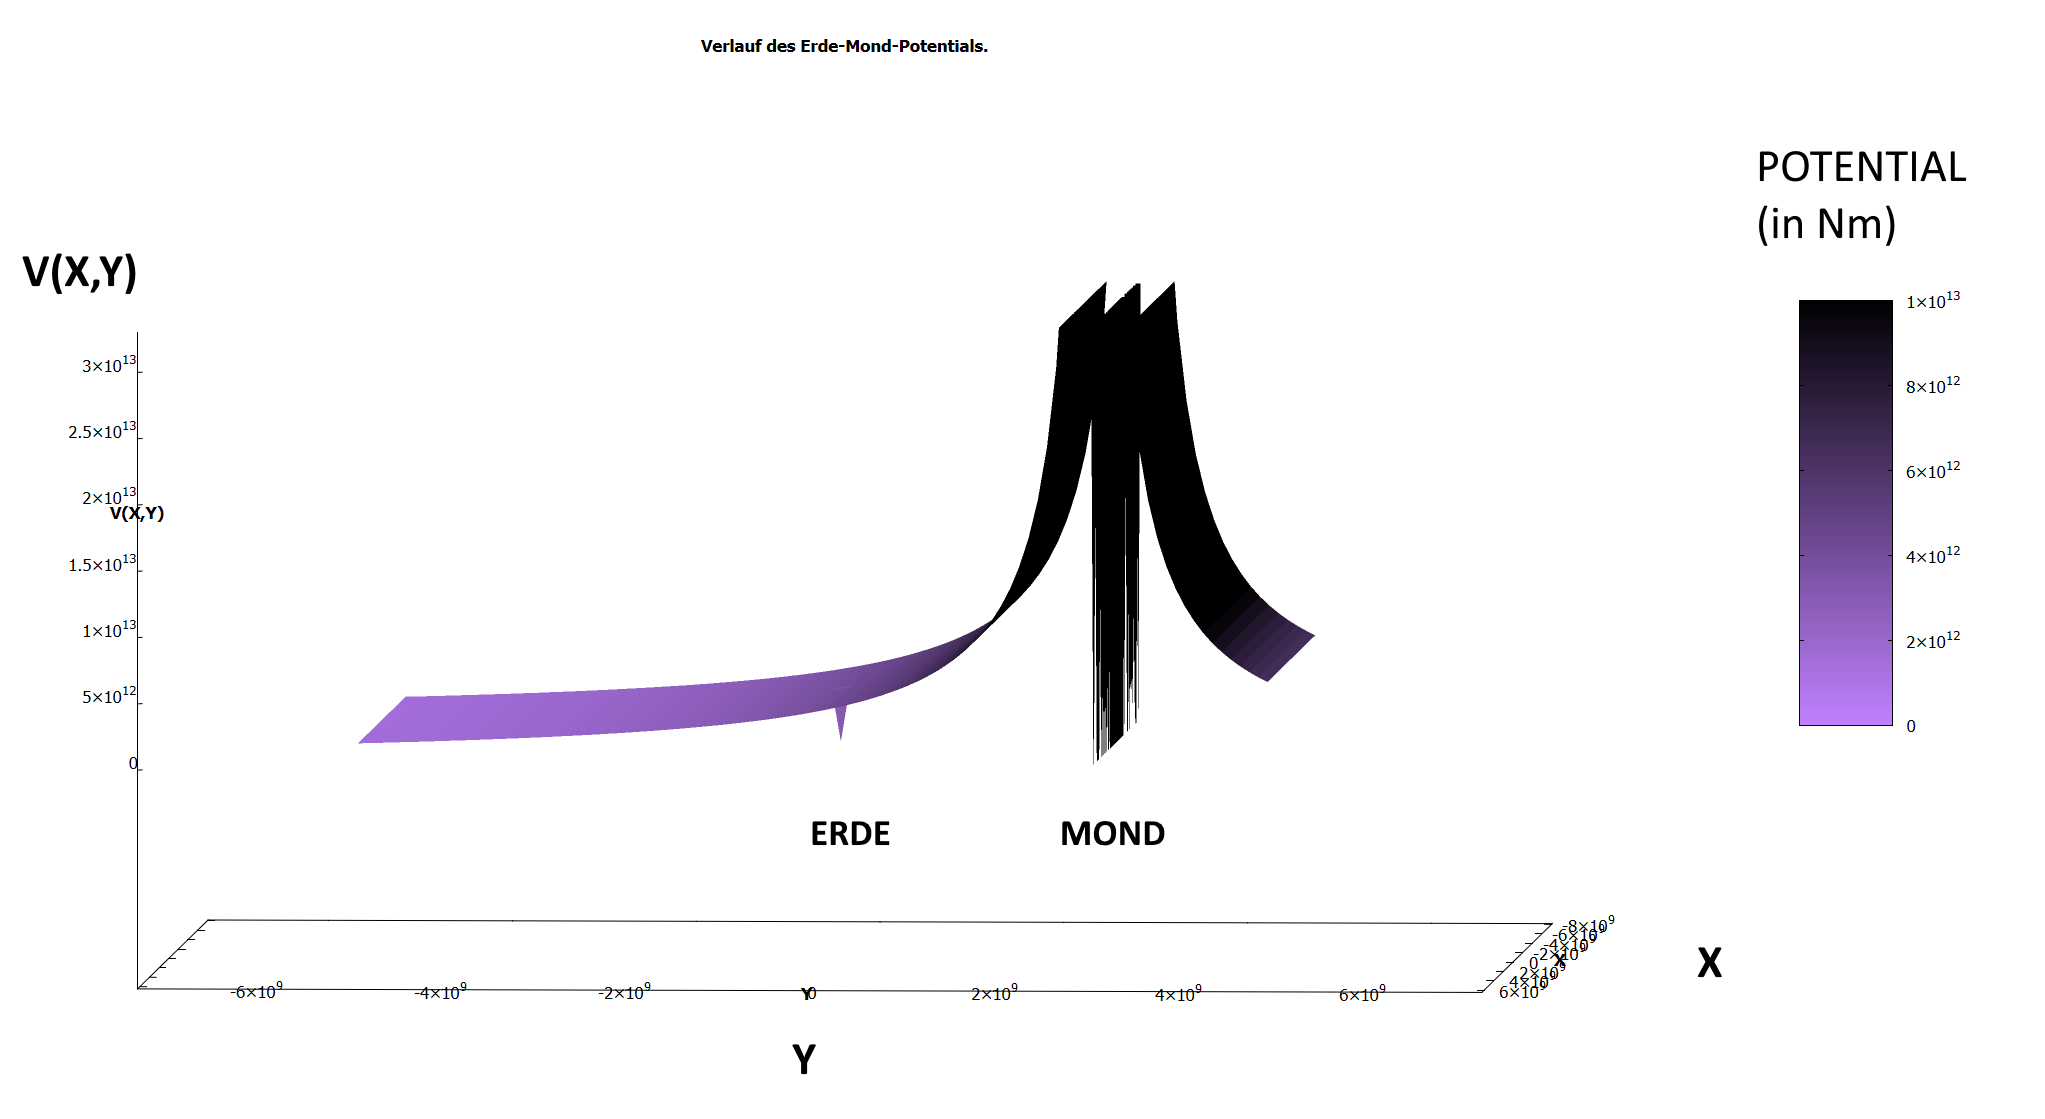
\includegraphics[width=0.8\textwidth]{../Ressource/PotentialVerlaufKugel.png}
        \caption{Potentialverlauf}
        \label{fig:Potential}
    \end{figure}
\end{document}